\documentclass[11pt]{article}

\usepackage[margin=1in]{geometry}
\usepackage[numbers]{natbib}


\usepackage{amsmath,amssymb,amsthm}
\usepackage{enumitem}
\usepackage{mathrsfs}
\usepackage{xcolor}
\usepackage{mathtools}
\usepackage{hyperref}
\usepackage[normalem]{ulem}

\usepackage{tikz}
\usepackage{tikz-cd}
\usetikzlibrary{arrows.meta, positioning, cd}
\usepackage{float}

\newtheorem{definition}{Definition}
\newtheorem{assumption}{Assumption}
\newtheorem{lemma}{Lemma}
\newtheorem{proposition}{Proposition}
\newtheorem{theorem}{Theorem}
\newtheorem{remark}{Remark}
\newtheorem{corollary}{Corollary}
\newtheorem{conjecture}{Conjecture}

\newcommand{\Rcal}{\mathcal{R}}
\newcommand{\Pcal}{\mathcal{P}}
\newcommand{\Mcal}{\mathcal{M}}
\newcommand{\Ncal}{\mathcal{N}}
\newcommand{\Fcal}{\mathcal{F}}
\newcommand{\Bcal}{\mathcal{B}}
\newcommand{\Xcal}{\mathcal{X}}
\newcommand{\Dcal}{\mathcal{D}}

\newcommand{\Psf}{\mathsf{P}}
\newcommand{\Lsf}{\mathsf{L}}
\newcommand{\Rsf}{\mathsf{R}}

\newcommand{\push}{\sharp}     	% pushforward
\newcommand{\Ext}{\mathrm{Ext}} 	% extension

\newcommand{\R}{\mathbb{R}}
\newcommand{\Pbb}{\mathbb{P}}
\newcommand{\Ebb}{\mathbb{E}} 	% expectation 
\newcommand{\Fib}{\mathrm{Fib}} 	% compatibility fibre

\title{Observable Dynamics: A Program}
\author{}
\date{}

\pagecolor{white}


\begin{document}
\maketitle

%%%%%%%%%%%%%%%%%%%%%%%%%%%%%%%%%%%%%%%%%%%%%%%%%%%%%%%%%%%%%%%%%%%%%
% Program overview
%%%%%%%%%%%%%%%%%%%%%%%%%%%%%%%%%%%%%%%%%%%%%%%%%%%%%%%%%%%%%%%%%%%%%

\section{Program overview}

This document outlines a research program in which probabilistic,
predictive, and dynamical structures are derived from observable
experiments rather than assumed as primitive properties of an
underlying state space.

The central thesis of the program is that the structures traditionally
treated as foundational in probability and dynamical systems—states,
laws, and dynamical evolution—may instead arise as consequences of
observable compatibility and predictive organization.

In this perspective, observable experiments play the primary role,
while probabilistic representations and dynamical structures appear as
derived organizational principles.

\paragraph{Program scope.}
The goal of the observable dynamics program is not to replace
classical probability or dynamical systems, but to provide an
observational foundation from which probabilistic, predictive, and
dynamical structure may arise as consequences of compatibility and
prediction.

Classical formulations of probability and dynamical systems typically
begin with a state space together with laws or evolution rules
defined on that space.  Observables are then treated as functions of
the state.  The present framework reverses this order of explanation.
We begin with a class of admissible observational queries and their
empirical regularities, and ask when probabilistic, predictive, and
dynamical structures become unavoidable.

At a high level the program has the following architecture

\begin{align*}
&\text{observable experiments}
\;\longrightarrow\;
\text{probabilistic representation}\\
&\qquad\longrightarrow\;
\text{predictive state space}
\;\longrightarrow\;
\text{predictive operators}.
\end{align*}

More concretely, starting from a query system

\[
(\mathcal Q,\preceq),
\]

the foundational results show that compatible observable experiments
admit a canonical probabilistic realization

\[
(\Omega,\sigma(\mathcal Q),P).
\]

Prediction then induces an equivalence relation on observable
configurations yielding a minimal predictive query

\[
Q_*,
\]

whose states correspond to distinct predictive laws of future
observables.  Predictive evolution is then described by operators

\[
(K_{Q_*} g)(q)=\mathbb E[g(F)\mid Q_*=q].
\]

Thus the core mathematical spine of the program is

\[
(\mathcal Q,\preceq)
\longrightarrow
(\Omega,P)
\longrightarrow
Q_*
\longrightarrow
K_{Q_*}.
\]


%%%%%%%%%%%%%%%%%%%%%%%%%%%%%%%%%%%%%%%%%%%%%%%%%%%%%%%%%%%%%%%%%%%%%
% Program structure diagram
%%%%%%%%%%%%%%%%%%%%%%%%%%%%%%%%%%%%%%%%%%%%%%%%%%%%%%%%%%%%%%%%%%%%%

\section{Program architecture}

The observable dynamics program develops dynamical structure directly
from observable experiments.  The program proceeds through three
conceptual stages.

\[
\begin{aligned}
&\textbf{Stage 1: Observational foundations} \\[6pt]
&\text{observable queries}
\;\longrightarrow\;
\text{compatibility structure}
\;\longrightarrow\;
\text{canonical experiment }(\Omega,\sigma(\mathcal{Q}),P)
\end{aligned}
\]

\begin{center}
Paper: \emph{Observational Foundations of Probability}
\end{center}

\vspace{8pt}

\[
\begin{aligned}
&\textbf{Stage 2: Predictive structure} \\[6pt]
&(\Omega,P)
\;\longrightarrow\;
\text{predictive kernels}
\;\longrightarrow\;
\text{predictive equivalence}
\;\longrightarrow\;
\text{minimal predictive query }Q_*
\end{aligned}
\]

\begin{center}
Paper: \emph{Predictive Experiments and Observable Operators}
\end{center}

\vspace{8pt}

\[
\begin{aligned}
&\textbf{Stage 3: Observable operator dynamics} \\[6pt]
&Q_*
\;\longrightarrow\;
\text{predictive operator }K_{Q_*}
\;\longrightarrow\;
\text{observable dynamical systems}
\end{aligned}
\]

\begin{center}
Future work: observable operator theory
\end{center}

\paragraph{Formal verification.}
The structural components of the observational framework are
formalized in Lean via the QuerySystem library, which defines query
systems, refinement maps, and the projective construction of the
canonical experiment.  This formalization ensures that the core
representation results are mechanically verified.

In summary, the program studies how dynamical structure can be derived
directly from observable experiments, progressing from observational
compatibility to probabilistic representation, predictive state
spaces, and finally observable operator dynamics.

\section{Structure of the observable dynamics program}

The observable dynamics program has a central theoretical spine together
with complementary formal and constructive branches, as summarized in
Figure~\ref{fig:observable-dynamics-program}.

\begin{figure}[H]
\centering
\resizebox{0.72\linewidth}{!}{%
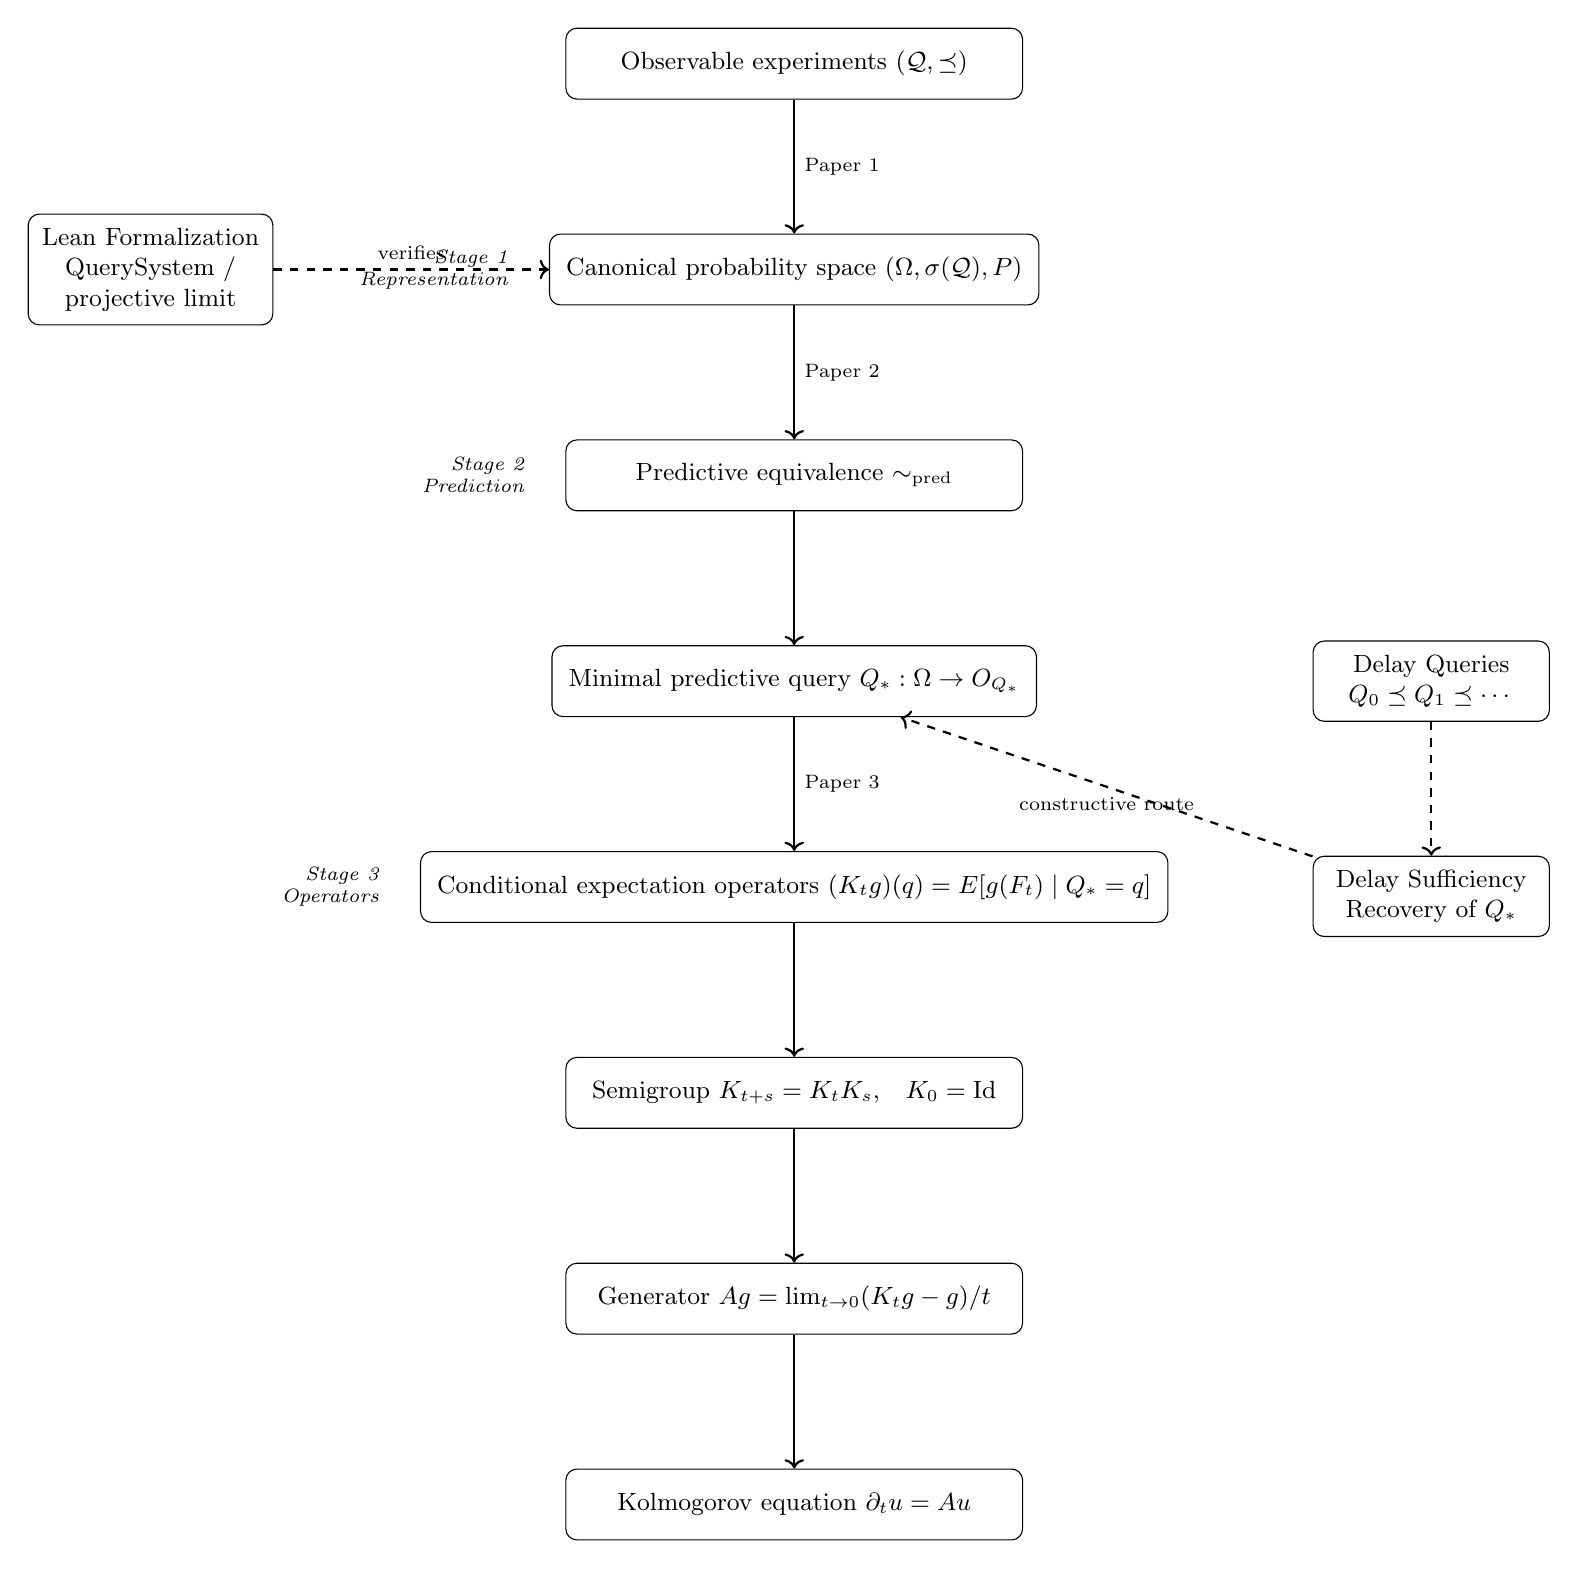
\begin{tikzpicture}[
    node distance=1.7cm and 3.2cm,
    box/.style={
        rectangle, draw, rounded corners,
        minimum width=5.8cm, minimum height=0.9cm,
        align=center, font=\small, inner sep=6pt
    },
    sidebox/.style={
        rectangle, draw, rounded corners,
        minimum width=3.0cm, minimum height=0.85cm,
        align=center, font=\small, inner sep=5pt
    },
    arrow/.style={->,thick},
    dashedarrow/.style={->,thick,dashed}
]

% Main vertical spine
\node[box] (queries) {Observable experiments $(\mathcal Q,\preceq)$};
\node[box, below=of queries] (prob)    {Canonical probability space $(\Omega,\sigma(\mathcal Q),P)$};
\node[box, below=of prob]    (equiv)   {Predictive equivalence $\sim_{\mathrm{pred}}$};
\node[box, below=of equiv]   (state)   {Minimal predictive query $Q_*:\Omega\to O_{Q_*}$};
\node[box, below=of state]   (ops)     {Conditional expectation operators $(K_t g)(q)=E[g(F_t)\mid Q_*=q]$};
\node[box, below=of ops]     (sg)      {Semigroup $K_{t+s}=K_t K_s$,\quad $K_0=\mathrm{Id}$};
\node[box, below=of sg]      (gen)     {Generator $Ag=\lim_{t\to0}(K_t g - g)/t$};
\node[box, below=of gen]     (kolm)    {Kolmogorov equation $\partial_t u = Au$};

% Side: Lean formalization (left)
\node[sidebox, left=3.5cm of prob] (lean)
    {Lean Formalization\\QuerySystem /\\projective limit};

% Side: delay embeddings (right)
\node[sidebox, right=3.5cm of state] (delay)
    {Delay Queries\\$Q_0\preceq Q_1\preceq\cdots$};
\node[sidebox, below=of delay] (takens)
    {Delay Sufficiency\\Recovery of $Q_*$};

% Main spine arrows
\draw[arrow] (queries) -- node[right,font=\scriptsize]{Paper 1} (prob);
\draw[arrow] (prob)    -- node[right,font=\scriptsize]{Paper 2} (equiv);
\draw[arrow] (equiv)   --                                       (state);
\draw[arrow] (state)   -- node[right,font=\scriptsize]{Paper 3} (ops);
\draw[arrow] (ops)     --                                       (sg);
\draw[arrow] (sg)      --                                       (gen);
\draw[arrow] (gen)     --                                       (kolm);

% Side arrows
\draw[dashedarrow] (lean)   -- node[above,font=\scriptsize]{verifies} (prob);
\draw[dashedarrow] (delay)  -- (takens);
\draw[dashedarrow] (takens) -- node[below,font=\scriptsize]{constructive route} (state);

% Stage labels (left of spine)
\node[left=0.4cm of prob,  align=right, font=\scriptsize\itshape] {Stage 1\\Representation};
\node[left=0.4cm of equiv, align=right, font=\scriptsize\itshape] {Stage 2\\Prediction};
\node[left=0.4cm of ops,   align=right, font=\scriptsize\itshape] {Stage 3\\Operators};

\end{tikzpicture}
}% end resizebox

\caption{Derivational spine of the observable dynamics program.
The main chain runs from observable queries through the canonical
probability space, predictive equivalence, and the minimal predictive
query $Q_*$, to the operator semigroup $\{K_t\}$, its generator $A$,
and the Kolmogorov evolution equation.
Lean formalization verifies the foundational layer (left).
Delay-query constructions provide a constructive route to $Q_*$ (right).}
\label{fig:observable-dynamics-program}

\end{figure}

\begin{center}
\textit{Observations $\rightarrow$ Probability $\rightarrow$ Prediction $\rightarrow$ State $\rightarrow$ Dynamics}
\end{center}

Observable experiments generate a probabilistic representation.
Prediction then induces a minimal predictive state space, and
predictive dynamics are represented by operators acting on functions
of that state space.

Figure~\ref{fig:observable-dynamics-program} displays the core architecture of the
program.  The first paper constructs probability from observable
compatibility, the second constructs predictive state spaces from the
canonical experiment, and the third develops the resulting operator
dynamics.

In this sense the program is organized by a single structural
progression:
\[
\text{observations}
\;\longrightarrow\;
\text{probability}
\;\longrightarrow\;
\text{prediction}
\;\longrightarrow\;
\text{state}
\;\longrightarrow\;
\text{dynamics}.
\]


\section{Program Theorems}

The long-term goal of the observable dynamics program is to establish a
sequence of structural theorems connecting observational experiments,
probabilistic representations, predictive state spaces, and operator
dynamics.  These theorems form the backbone of the theory.

\subsection{Observational completion}

\begin{theorem}[Observational Completion Theorem]
Let $(\mathcal Q,\preceq)$ be a compatible system of observable queries
with associated observable laws $\{\nu_Q\}_{Q\in\mathcal Q}$.

Under suitable compatibility conditions there exists a probability
space
\[
(\Omega,\sigma(\mathcal Q),P)
\]
such that for every query $Q$
\[
Q_\#P=\nu_Q .
\]

Thus compatible observable experiments admit a canonical probabilistic
representation.
\end{theorem}

This theorem establishes the transition

\[
\text{observable experiments}
\rightarrow
\text{probabilistic representation}.
\]

\subsection{Predictive state realization}

\begin{theorem}[Predictive State Realization]
Let $(\Omega,P)$ be the canonical observational experiment.

For any future observable $F$ define predictive equivalence

\[
q\sim q'
\quad\Longleftrightarrow\quad
P(F\in\cdot \mid q)
=
P(F\in\cdot \mid q').
\]

Under suitable regularity conditions the predictive equivalence
classes form a standard Borel space $Q_*$ and the conditional law of
the future observable factors through this space.
\end{theorem}

This theorem establishes the transition

\[
\text{probabilistic representation}
\rightarrow
\text{predictive state space}.
\]

\subsection{Predictive minimality}

\begin{theorem}[Predictive Minimality]
The predictive state space $Q_*$ is minimal among all observable
representations that retain the predictive law of the future observable
$F$.

In particular, if $Q$ is predictively sufficient then there exists a
measurable map
\[
Q\to Q_*.
\]
\end{theorem}

Thus the predictive state space may be interpreted as the minimal
observable sufficient statistic for prediction.

\subsection{Predictive operator realization}

\begin{theorem}[Predictive Operator Realization]
Let $Q_*$ be the predictive state space.

For bounded measurable functions $g$ define
\[
(K_{Q_*}g)(q)
=
\mathbb E[g(F)\mid Q_*=q].
\]

Then $K_{Q_*}$ defines a positive linear operator acting on functions
of the predictive state space.  Predictive evolution of observable
expectations is represented entirely through this operator.
\end{theorem}

This establishes the transition

\[
\text{predictive states}
\rightarrow
\text{operator dynamics}.
\]

\subsection{Observable dynamics closure}

\begin{theorem}[Observable Dynamics Closure]
Under suitable conditions the pair

\[
(Q_*,K_{Q_*})
\]

completely characterizes the predictive evolution of observable
quantities.  In this sense observable dynamical laws are equivalent to
operator dynamics acting on the predictive state space.
\end{theorem}

This theorem expresses the central claim of the program: observable
dynamics may be represented entirely through predictive operators on
predictive state spaces.

%%%%%%%%%%%%%%%%%%%%%%%%%%%%%%%%%%%%%%%%%%%%%%%%%%%%%%%%%%%%%%%%%%%%%
% Structural principles
%%%%%%%%%%%%%%%%%%%%%%%%%%%%%%%%%%%%%%%%%%%%%%%%%%%%%%%%%%%%%%%%%%%%%

\section{Structural principles}

The observable-dynamics program is guided by several structural
principles.

\begin{itemize}

\item \textbf{Completion principle.}
Families of compatible observable experiments admit probabilistic
representations.

\item \textbf{Predictive sufficiency principle.}
Prediction induces minimal observable state spaces capturing exactly
the predictive information relevant to future observables.

\item \textbf{Operator representation principle.}
Predictive evolution admits operator-theoretic representations on
predictive state spaces.

\item \textbf{Forcing principle.}
Compatibility constraints among observable regularities may force
structural relations among observables.

\item \textbf{Universality principle.}
Distinct underlying mechanisms may exhibit identical observable
regularities relative to a given query system.

\end{itemize}


%%%%%%%%%%%%%%%%%%%%%%%%%%%%%%%%%%%%%%%%%%%%%%%%%%%%%%%%%%%%%%%%%%%%%
% Program conjectures
%%%%%%%%%%%%%%%%%%%%%%%%%%%%%%%%%%%%%%%%%%%%%%%%%%%%%%%%%%%%%%%%%%%%%

\section{Program conjectures}

The following conjectures articulate the central structural claims of
the observable-dynamics program.  They describe mechanisms through
which probabilistic, predictive, and dynamical structure may emerge
from observable experiments.

These conjectures should be interpreted as organizing principles for
future research rather than as immediate theorems.

\begin{conjecture}[Predictive state emergence]
For sufficiently rich query systems admitting a probabilistic
completion $(\Omega,P)$, predictive equivalence induces a minimal
predictive query
\[
Q_*,
\]
whose states correspond to distinct conditional laws of future
observables.
\end{conjecture}

%%%%%%%%%%%%%%%%%%%%%%%%%%%%%%%%%%%%%%%%%%%%%%%%%%%%%%%%%%%%%%%%%%%%%

\begin{conjecture}[Predictive minimal sufficiency]
\label{conj:predictive-minimal-sufficiency}

Let $(\Omega,\sigma(\mathcal Q),P)$ be the probabilistic
representation associated with a query system, and let $F$ be a future
observable.

Then the minimal predictive query $Q_*$ is the observable analogue of
a minimal sufficient statistic for predicting $F$.

More precisely:

\begin{enumerate}

\item the conditional law
\[
P(F\in\cdot \mid \text{present observable configuration})
\]
factors through $Q_*$;

\item any other predictively sufficient query factors through $Q_*$
up to predictive equivalence;

\item $Q_*$ is unique up to measurable isomorphism of predictive
state spaces.

\end{enumerate}

\end{conjecture}

\begin{remark}
This conjecture places predictive state formation in direct analogy
with classical sufficiency theory.  The predictive state space $Q_*$
is not an assumed latent state but an observable quotient preserving
all information relevant for predicting the future observable $F$.

In this sense predictive states arise as organizational summaries of
observable configurations rather than as hidden microscopic variables.
\end{remark}

%%%%%%%%%%%%%%%%%%%%%%%%%%%%%%%%%%%%%%%%%%%%%%%%%%%%%%%%%%%%%%%%%%%%%

\begin{conjecture}[Predictive operator representation]
Predictive evolution of observable quantities may be represented by a
positive linear operator
\[
K_{Q_*}
\]
acting on functions of the predictive state space.
\end{conjecture}


\begin{conjecture}[Predictive Koopman--Perron correspondence]

Let $Q_*$ be the predictive state space associated with a future
observable $F$ and

\[
(K_{Q_*} g)(q)=\mathbb E[g(F)\mid Q_*=q].
\]

Then predictive dynamics admit a dual operator acting on predictive
laws such that

\begin{enumerate}

\item deterministic systems recover classical Koopman and
Perron--Frobenius operators;

\item stochastic systems yield an observable operator representation of
predictive dynamics;

\item spectral properties of the predictive operator reflect ergodic
structure of the observable system.

\end{enumerate}

\end{conjecture}

\begin{conjecture}[Functoriality of predictive state spaces]
\label{conj:functorial-predictive-state}

Morphisms of observational systems that preserve predictive structure
induce structure-preserving maps between the corresponding minimal
predictive state spaces
\[
\Phi_* : Q_* \to Q_*'
\]
and intertwine their predictive operators in the appropriate sense.

Thus the assignment
\[
(\text{observational system})
\longmapsto
(\text{predictive state space})
\]
is expected to be functorial.
\end{conjecture}

\begin{remark}
This conjecture suggests that predictive state spaces are not isolated
constructions but belong to a broader category of observable dynamical
representations.  If true, it would connect the observational program
to categorical probability and functorial formulations of dynamics.
\end{remark}


\begin{conjecture}[Delay sufficiency principle]

For time-series observables satisfying mild regularity conditions,
increasing delay queries

\[
Q_0 \preceq Q_1 \preceq Q_2 \preceq \cdots
\]

eventually realize a predictively sufficient statistic.

\end{conjecture}


\begin{conjecture}[Universality of observable regularities]

Distinct microscopic mechanisms may produce identical observable
regularities relative to the same query system.

\end{conjecture}


\begin{conjecture}[Thermodynamic emergence]

Large-scale statistical laws such as entropy and thermodynamic
relations may arise from compatibility among observable experiments
across observational scales.

\end{conjecture}


\section{Motivation}

The preceding sections state the program at a structural level.  The
purpose of the present note is to explain why this reversal of
perspective is mathematically fruitful and why it leads naturally to a
broader theory of observable dynamics.

Classical probability, dynamics, and statistical mechanics are typically
formulated by starting from an assumed state space together with laws or
evolution rules defined on that space.  The observational framework
reverses this order of explanation.  One begins with a class of admissible
queries and their observable regularities, and asks when probabilistic,
predictive, and dynamical structure become unavoidable.

The broader question pursued here is what structures emerge once this
observational starting point is adopted.  These include recurrence and
forcing, universality, thermodynamic organization, operator-theoretic
structure, and exploratory applications to areas such as symbolic
dynamics, statistical mechanics, and number theory.

Throughout, we assume a class of admissible boundary queries
\[
\mathcal Q,
\]
and a corresponding family of observable regularities
\[
\{\nu_Q\}_{Q\in\mathcal Q}.
\]

No underlying path-space law or state-space dynamics is assumed.

\section{Program architecture}

\subsection{Foundational layer: observational probability}

The first paper of the program studies when a compatible family of
observable experiments admits a canonical probabilistic realization.
Schematically,
\[
(\mathcal Q,\preceq)
\;\longrightarrow\;
(\Omega,\sigma(\mathcal Q),P).
\]

Here $(\mathcal Q,\preceq)$ is a query system ordered by refinement,
while $(\Omega,\sigma(\mathcal Q),P)$ is the canonical probabilistic
representation whose query marginals recover the observed laws.

\subsection{Predictive layer: minimal predictive state spaces}

The second paper studies how predictive structure emerges once the
canonical experiment has been constructed.  Given a future observable,
one obtains predictive kernels, predictive equivalence, a minimal
predictive query $Q_*$, and predictive operators:
\[
(\Omega,\sigma(\mathcal Q),P)
\;\longrightarrow\;
Q_*
\;\longrightarrow\;
K_{Q_*}.
\]

Thus the first two papers establish the core pipeline
\[
\text{observations}
\;\longrightarrow\;
\text{probability}
\;\longrightarrow\;
\text{predictive state}
\;\longrightarrow\;
\text{predictive operators}.
\]

\subsection{Broader program directions}

Once this core architecture is in place, a number of additional research
directions become natural:
\begin{itemize}
\item recurrence and forcing,
\item universality and thermodynamic structure,
\item symbolic and information-theoretic hierarchies,
\item operator-theoretic formulations,
\item data-driven and number-theoretic applications.
\end{itemize}

\section{Next phase of the program}

The foundational paper and its predictive sequel establish the first
two structural layers of the observable dynamics program:

\begin{enumerate}
\item compatible observable experiments admit a canonical probabilistic
representation $(\Omega,P)$;
\item predictive structure on this representation yields predictive
kernels and predictive equivalence relations.
\end{enumerate}

The next phase of the program focuses on the deeper structural
properties of predictive states and predictive dynamics.  Three
problems appear particularly central.

\paragraph{Predictive state realization.}
The predictive equivalence relation
\[
q \sim q'
\quad\Longleftrightarrow\quad
P(F\in\cdot \mid q)=P(F\in\cdot \mid q')
\]
defines predictive states as equivalence classes of observable
configurations.  A fundamental problem is to establish conditions under
which these classes form a well-behaved measurable quotient space
$Q_*$.  Such a result would show that predictive states exist as
minimal observable representations preserving the predictive law of
future observables.

\paragraph{Predictive operator theory.}
Once predictive states are available, predictive evolution may be
represented by operators acting on functions of the predictive state
space:
\[
(K_{Q_*} g)(q)=\mathbb E[g(F)\mid Q_*=q].
\]
Developing the structure of these operators---their positivity,
semigroup properties, spectral behavior, and relations to classical
Koopman and Perron--Frobenius operators---forms a natural second stage
of the theory.

\paragraph{Observable recovery via delay queries.}
For time-series observables, delay queries generate an increasing
family of observable experiments
\[
Q_0\preceq Q_1\preceq Q_2\preceq\cdots .
\]
A central question is whether sufficiently rich delay observations
recover the minimal predictive state space.  Establishing such
``delay sufficiency'' results would connect the abstract theory with
practical observable reconstructions used in dynamical systems and
time-series analysis.

Together these problems aim to establish a complete chain
\[
(\mathcal Q,\preceq)
\;\longrightarrow\;
(\Omega,P)
\;\longrightarrow\;
Q_*
\;\longrightarrow\;
K_{Q_*},
\]
thereby providing an observational route from empirical experiments to
predictive state spaces and operator representations of observable
dynamics.

\section{Recurrence, forcing, and observable structure}

\subsection{Structural queries}

Let $Q\in\mathcal Q$ be a boundary query with outcome space $\mathcal O_Q$.
Typical examples include:
\begin{itemize}
\item finite-lag projections,
\item coarse-grained symbolic encodings,
\item delay embeddings,
\item partition-based observations.
\end{itemize}

Each query produces an observable regularity
\[
\nu_Q \in \mathcal P(\mathcal O_Q).
\]

\begin{definition}[Recurrence query]
A query $Q\in\mathcal Q$ is called a \emph{recurrence query} if its outcome
space admits a natural notion of recurrence, such as:
\begin{itemize}
\item periodic symbolic patterns,
\item return times,
\item invariant or recurrent subsets,
\item shift-invariant symbolic structures.
\end{itemize}
\end{definition}

\begin{remark}
The definition is intentionally broad. The notion of recurrence is determined
by the observational protocol rather than a privileged state-space structure.
\end{remark}

\subsection{Observable recurrence structures}

Let $\mathcal S_Q$ denote a collection of structural properties of
$\nu_Q$ corresponding to recurrence phenomena. Examples include:
\begin{itemize}
\item existence of a periodic pattern of length $n$,
\item positive entropy,
\item mixing,
\item existence of a subshift factor.
\end{itemize}

\begin{definition}[Query-detectable structure]
A recurrence structure $S\in\mathcal S_Q$ is said to be
\emph{query-detectable} if it depends only on the observable regularity
$\nu_Q$ and not on any interior realization.
\end{definition}

\begin{remark}
This ensures that recurrence is defined empirically, rather than as a
property of a particular dynamical model.
\end{remark}

\section{Boundary forcing and structural hierarchies}

We now define a forcing relation among observable recurrence structures.

\begin{definition}[Boundary forcing]
Let $S_1,S_2$ be query-detectable recurrence structures (possibly arising
from different queries). We say that
\[
S_1 \;\Rightarrow\; S_2
\]
(\emph{$S_1$ boundary-forces $S_2$}) if the following holds:

For every boundary horizon $\{\nu_Q\}$ that admits a completion compatible
with the observed queries and satisfies structure $S_1$, every such completion
also satisfies $S_2$.
\end{definition}

\begin{remark}
This relation depends only on observable regularities and their
extendability, not on any assumed dynamical law.
\end{remark}

\begin{remark}
Boundary forcing is therefore:
\begin{itemize}
\item query-relative,
\item resolution-relative,
\item independent of dimension,
\item independent of state-space smoothness.
\end{itemize}
\end{remark}

\begin{remark}[Relation to predictive state structure]
Within the broader observational program, boundary forcing may be
interpreted as a structural constraint on admissible predictive
representations.  In particular, forcing relations restrict the
possible predictive state spaces and predictive operators that can
arise from a given family of observable regularities.
\end{remark}

\section{Classical and higher-dimensional recurrence applications}

\begin{definition}[Structural hierarchy]
The partial order induced by boundary forcing defines a hierarchy of
observable recurrence structures:
\[
S_1 \Rightarrow S_2.
\]
\end{definition}

This generalizes classical forcing relations in dynamical systems.

\begin{proposition}
Boundary forcing is transitive and reflexive.
\end{proposition}

\begin{proof}
Reflexivity is immediate.

If $S_1 \Rightarrow S_2$ and $S_2 \Rightarrow S_3$, then any compatible
completion exhibiting $S_1$ exhibits $S_2$, and therefore $S_3$.
\end{proof}

\section{Classical Sharkovskii ordering as a special case}

We now show that the classical Sharkovskii theorem fits into this framework.

Let $Y=[0,1]$ and consider discrete maps
\[
f:Y\to Y.
\]

Choose a partition-based symbolic query:
\[
Q:\text{orbit} \mapsto \text{symbolic itinerary}.
\]

Define structures:
\begin{itemize}
\item $S_n$: existence of a symbolic periodic pattern of period $n$.
\end{itemize}

\begin{theorem}[Sharkovskii as boundary forcing]
In one-dimensional interval dynamics, the classical Sharkovskii ordering
corresponds to a boundary forcing hierarchy among symbolic periodic
structures.
\end{theorem}

\begin{remark}
This interpretation does not depend on differentiability or smoothness,
but only on observable symbolic recurrence.
\end{remark}

\section{Higher-dimensional generalization}

In higher dimensions, periodicity alone is insufficient to capture forcing.
Instead, the relevant structures include:
\begin{itemize}
\item subshifts of finite type,
\item topological entropy,
\item invariant symbolic factors,
\item braid or homological recurrence.
\end{itemize}

\begin{definition}[Symbolic dominance]
We say that structure $S_1$ symbolically dominates $S_2$ if any observable
realization of $S_1$ induces $S_2$ under the same query class.
\end{definition}

This leads to a generalized Sharkovskii-type hierarchy based on symbolic and
information-theoretic structure rather than period alone.

\section{Universality, equilibrium, and thermodynamic structure}

The next layer of the program concerns the emergence of large-scale
statistical organization from compatibility and completion constraints.
The main idea is that familiar structures such as equilibrium,
universality, and thermodynamic behavior may be interpreted as
consequences of observable consistency rather than as primitive
assumptions.

\subsection{Program directions}

This part of the program includes:
\begin{itemize}
\item query-relative entropy hierarchies,
\item information-geometric forcing,
\item statistical-mechanical interpretations of recurrence,
\item empirical detection of structural transitions.
\end{itemize}

In particular, the boundary completion framework suggests that structural
forcing is fundamentally a question of extendability across resolutions.

\subsection{Exploratory application: the Riemann zeta function}
\label{sec:zeta-program}

This note outlines a possible research program for applying the boundary-query
framework to number-theoretic structures, with particular focus on the Riemann
zeta function. The intent is exploratory: no structural assumptions are imposed
a priori, and all dynamical or operator structure is treated as derived.

\subsection{Motivation}

The Riemann zeta function
\[
\zeta(s) = \prod_{p} (1 - p^{-s})^{-1}
\]
admits a formal analogy with dynamical zeta functions arising in chaotic systems,
where periodic orbits replace prime numbers. This suggests the possibility of an
underlying dynamical or statistical structure. However, most existing approaches
assume such a structure in advance.

Within the observational program, one may instead ask whether dynamical
or operator-theoretic structure could emerge from observable
regularities of prime statistics across scales.

\subsection{Observable regularities of prime sequences}

Let $\mathbb{P}$ denote the ordered sequence of prime numbers. Rather than
starting with an analytic function, we consider a class of observable queries
$\mathcal{Q}$ acting on this sequence.

Examples include:
\begin{itemize}
  \item Gap statistics: distributions of $p_{n+1} - p_n$.
  \item Local correlation functions.
  \item Windowed prime-count statistics.
  \item Spectral statistics of truncated Dirichlet series.
  \item Symbolic encodings of primes.
\end{itemize}

For each query $Q \in \mathcal{Q}$, we define a set of admissible empirical
regularities $\mathcal{R}_Q$. A boundary horizon is then a family
\[
\{\nu_Q\}_{Q \in \mathcal{Q}}, \qquad \nu_Q \in \mathcal{R}_Q,
\]
interpreted as the observable regularities of the prime sequence at various
scales.

\subsection{Boundary completion across scales}

We ask whether these observable regularities admit approximate extension across
scales. In particular, for queries defined at resolutions $n$ and $m$, we study
whether joint realizability holds:
\[
\nu_{Q_{n+m}} \approx \mathrm{Ext}(\nu_{Q_n}, \nu_{Q_m}).
\]

Failure of such completion identifies regimes where multi-scale prime
statistics cannot be consistently unified.

Approximate completion provides a quantitative measure of coherence across
scales and may be related to conjectures such as:
\begin{itemize}
  \item Montgomery pair correlation.
  \item Random matrix universality.
  \item Distribution of zeros.
\end{itemize}

\subsection{Statistical forcing and universality}

A central question is whether certain low-resolution regularities force
higher-order structure. For example:
\begin{itemize}
  \item Do local gap statistics constrain long-range correlations?
  \item Is random-matrix behavior forced by compatibility across scales?
\end{itemize}

This suggests the possibility of forcing hierarchies among observable
prime statistics analogous to recurrence hierarchies in dynamical
systems.

\subsection{Emergence of transfer operators}

If boundary regularities admit suitable disintegrations, it may be
possible to obtain kernel-based predictive representations:

\[
T_{\Delta t} : \mathcal{X} \leadsto \mathcal{X},
\]
leading potentially to transfer-operator formulations.

The key point is that such operators are not assumed but derived. This may
provide a pathway toward:
\begin{itemize}
  \item Spectral interpretations of $\zeta$.
  \item Connections to the Hilbert--Pólya conjecture.
  \item Thermodynamic formalism for primes.
\end{itemize}

\subsection{Non-equilibrium statistical mechanics viewpoint}

From the present perspective, the zeta function may be viewed as encoding
multi-scale regularities of the prime sequence rather than solely as an
analytic object.

This connects to:
\begin{itemize}
  \item Large deviation theory.
  \item Entropy and information flow.
  \item Renormalization and scaling.
\end{itemize}

One speculative possibility is that classical conjectures such as the
Riemann hypothesis could correspond to structural stability conditions
for multi-scale compatibility of observable regularities.

\subsection{Initial concrete program}

A feasible first project is the study of approximate boundary completion for
prime gap statistics:
\begin{enumerate}
  \item Define a hierarchy of finite-resolution queries.
  \item Measure extension consistency across scales.
  \item Compare with predictions from random matrix theory.
\end{enumerate}

Such investigations may clarify which statistical regularities are fundamental
and which emerge as consequences of multi-scale compatibility.

\subsection{Outlook}

This perspective aims to unify number theory, statistical mechanics, and
dynamical systems within a common empirical framework. The goal is not to impose
dynamics on prime structure but to determine when and how such dynamics become
unavoidable.

Further directions include:
\begin{itemize}
  \item Higher-dimensional symbolic models of primes.
  \item Connections to quantum chaos.
  \item Operator-theoretic constructions guided by boundary completion.
\end{itemize}

\section{Universality and thermodynamic structure}

We now outline how large-scale statistical and dynamical structure may arise
as consequences of compatibility and extension constraints on boundary
regularities.  The viewpoint adopted here is that familiar notions such as
equilibrium, universality, and thermodynamic behavior need not be assumed a
priori, but may instead emerge as consequences of boundary consistency.

\subsection{Boundary forcing}

\begin{remark}[Structural forcing viewpoint]
The concept of boundary forcing introduced earlier may be interpreted
more generally as a structural principle: compatibility constraints
among observable regularities restrict the class of admissible
realizations.  In this way, dynamical or thermodynamic structure may
appear as a necessary consequence of empirical consistency rather than
as a modeling assumption.
\end{remark}

Typical examples of structural properties include:
\begin{itemize}
  \item existence of kernel representations,
  \item approximate semigroup structure,
  \item existence of a generator,
  \item mixing or ergodic behavior,
  \item scaling or universality properties.
\end{itemize}

Thus, dynamics appears not as a primitive assumption but as a necessary
consequence of compatibility among observable regularities.

\begin{remark}[Forcing versus modeling]
Boundary forcing is independent of modeling choices.
It identifies structural features that are unavoidable once empirical
constraints are imposed.
\end{remark}

\subsection{Universality as stability of boundary structure}

Universality refers to the empirical phenomenon that distinct microscopic
models produce indistinguishable large-scale statistical behavior.
Within the present framework, this is interpreted as stability of boundary
regularities under admissible realizations.

\begin{definition}[Boundary universality]
A class of realizations is said to exhibit \emph{boundary universality} if
they induce the same boundary regularities for a specified class of queries.
\end{definition}

This viewpoint shifts emphasis from interior structure to observable
regularities.  Universality emerges when extension and compatibility
constraints restrict the admissible boundary families to a small set.

\begin{remark}
Universality therefore reflects non-uniqueness of interior realizations
consistent with the same boundary horizon.
\end{remark}

\subsection{Equilibrium as exact boundary completion}

Exact boundary completion across resolutions provides a natural notion of
equilibrium.

\begin{definition}[Equilibrium boundary horizon]
A boundary horizon is said to be in \emph{equilibrium} if the associated
boundary family is exactly complete across all resolutions.
\end{definition}

In this case, finite-resolution regularities are mutually consistent and
admit coherent extension at all scales.

Conversely, deviations from equilibrium correspond to structured failure of
boundary completion.

\begin{remark}[Non-equilibrium regimes]
Non-equilibrium behavior may be interpreted as persistent incompatibility of
boundary regularities across resolutions.
Such incompatibility can arise even when each individual scale appears
well-behaved.
\end{remark}

\subsection{Approximate completion and large deviations}

Approximate boundary completion naturally leads to a large deviation
interpretation of empirical incompatibility.

Let $\varepsilon$ denote the minimal divergence required to reconcile
boundary regularities across scales.
Then $\varepsilon$ may be interpreted as a cost of enforcing consistency.

\begin{definition}[Boundary rate function]
A rate function associated with boundary incompatibility is defined by
\[
I := \inf_{\widetilde\Gamma \in \Ext(\Gamma_1,\Gamma_2)}
D_f(\Gamma_{12},\widetilde\Gamma),
\]
where $\Gamma_{12}$ denotes an observed long-lag regularity.
\end{definition}

This quantity measures the minimal empirical cost of reconciling observed
regularities with a jointly realizable structure.

\begin{remark}
This interpretation connects boundary completion with large deviation theory.
Compatibility corresponds to zero cost, while deviations correspond to
rare or constrained behavior.
\end{remark}

\subsection{Thermodynamic formalism as an emergent structure}

Thermodynamic formalism arises when boundary forcing selects a preferred
class of compatible realizations.

In particular:
\begin{itemize}
  \item entropy quantifies multiplicity of compatible realizations,
  \item free energy reflects trade-offs between compatibility and constraint,
  \item equilibrium measures maximize compatibility subject to constraints.
\end{itemize}

Thus, thermodynamic structure is interpreted as an optimization principle
arising from empirical consistency rather than as an intrinsic property of
a predefined dynamical system.

\begin{remark}[Maximum entropy and least action]
Principles such as maximum entropy and least action may be viewed as
selection criteria among admissible realizations that maintain compatibility
across scales.
\end{remark}

\subsection{Toward universality classes of boundary horizons}

A long-term goal of this framework is to classify boundary horizons according
to their forcing and universality properties.

Such a classification would parallel:
\begin{itemize}
  \item phase transitions in statistical mechanics,
  \item universality classes in critical phenomena,
  \item invariant structures in dynamical systems.
\end{itemize}

In this sense, the boundary horizon provides a common language for relating
empirical regularities, statistical structure, and dynamical representations.

% ============================================================
% Formal categorical scaffolding for the query/compatibility framework
% (with explicit category definitions + commutative diagrams)
% ============================================================
%
% Requires:
% \usepackage{amsmath,amssymb,amsthm}
% \usepackage{tikz-cd}
%
% The intent here is to make the “sits between” claim precise:
%   (i) classical probability spaces (state/event primitive),
%   (ii) observational/query systems (maps primitive),
%   (iii) a completion construction as a functor (under hypotheses).
%
% NOTE: I write everything in a standard-Borel setting to avoid pathologies.
% ============================================================

% ---------------------------
% Basic categories
% ---------------------------

\section{Technical scaffolding for the program}

The preceding sections describe the conceptual program and several
application families.  The present section records a possible categorical
organization of the framework.  Its role is not to drive the main
narrative of the note, but to clarify how the observational completion
construction sits between classical probabilistic models and more general
query-based observational specifications.

\subsection{Formal categorical scaffolding for the query/compatibility framework}

\begin{definition}[Category $\mathbf{Meas}$]
Objects are measurable spaces $(X,\Sigma_X)$. Morphisms are measurable maps
$f:(X,\Sigma_X)\to (Y,\Sigma_Y)$.
\end{definition}

\begin{definition}[Category $\mathbf{Prob}$]
Objects are pairs $(X,\mu)$ where $X$ is standard Borel and $\mu\in\mathcal P(X)$.
A morphism $(X,\mu)\to (Y,\nu)$ is a measurable map $f:X\to Y$ such that
$f_\#\mu=\nu$.
\end{definition}

\begin{definition}[Category $\mathbf{Stoch}$ (optional)]
Objects are standard Borel spaces. A morphism $X\leadsto Y$ is a Markov kernel
$K:X\times\mathcal B(Y)\to [0,1]$. Composition is kernel composition.
(Equivalently, $\mathbf{Stoch}$ is the Kleisli category of the Giry monad.)
\end{definition}

% ---------------------------
% Query systems as projective systems
% ---------------------------

\begin{definition}[Directed preorders and projective systems in $\mathbf{Meas}$]
Let $(\mathcal Q,\preceq)$ be a directed preorder (for any finite $Q_1,\dots,Q_n$
there exists $Q_\star$ with $Q_i\preceq Q_\star$).
A \emph{projective system of measurable spaces} indexed by $\mathcal Q$ is:
\begin{itemize}
\item objects $(O_Q,\mathcal B(O_Q))$ for each $Q\in\mathcal Q$,
\item measurable bonding maps $\pi^{Q_2}_{Q_1}:O_{Q_2}\to O_{Q_1}$ for $Q_1\preceq Q_2$,
\end{itemize}
satisfying identity and cocycle:
\[
\pi^{Q}_{Q}=\mathrm{id}_{O_Q},\qquad
\pi^{Q_3}_{Q_1}=\pi^{Q_2}_{Q_1}\circ \pi^{Q_3}_{Q_2}\quad(Q_1\preceq Q_2\preceq Q_3).
\]
\end{definition}

\begin{definition}[Compatible family of laws]
Given a projective system $\{O_Q,\pi\}$, a family $\{\nu_Q\}_{Q\in\mathcal Q}$ with
$\nu_Q\in\mathcal P(O_Q)$ is \emph{projectively compatible} if
\[
(\pi^{Q_2}_{Q_1})_\#\nu_{Q_2}=\nu_{Q_1}\qquad\forall\, Q_1\preceq Q_2.
\]
\end{definition}

\begin{remark}[The fundamental commutative square]
For $Q_1\preceq Q_2$, compatibility is the statement that the following diagram
commutes in $\mathbf{Prob}$:
\[
\begin{tikzcd}
(O_{Q_2},\nu_{Q_2}) \arrow[r,"\pi^{Q_2}_{Q_1}"] \arrow[dr,swap,"\mathrm{id}"]
& (O_{Q_1},\nu_{Q_1}) \arrow[d,"\mathrm{id}"] \\
& (O_{Q_1},\nu_{Q_1})
\end{tikzcd}
\qquad\text{equivalently}\qquad
(\pi^{Q_2}_{Q_1})_\#\nu_{Q_2}=\nu_{Q_1}.
\]
\end{remark}

% ---------------------------
% A category of "observational specifications"
% ---------------------------

\begin{definition}[Category $\mathbf{ObsSpec}$ of observational specifications]
An object is a triple
\[
\mathsf S = \big(\mathcal Q,\{O_Q\}_{Q\in\mathcal Q},\{\pi^{Q_2}_{Q_1}\}_{Q_1\preceq Q_2};\{\nu_Q\}_{Q\in\mathcal Q}\big)
\]
where $(\mathcal Q,\preceq)$ is directed, $\{O_Q,\pi\}$ is a projective system of standard Borel
spaces, and $\{\nu_Q\}$ is projectively compatible.

A morphism $\mathsf S\to \mathsf S'$ consists of:
\begin{itemize}
\item a monotone map $\alpha:(\mathcal Q,\preceq)\to (\mathcal Q',\preceq')$,
\item measurable maps $\theta_Q:O_Q\to O'_{\alpha(Q)}$ for each $Q$,
\end{itemize}
such that the squares commute for all $Q_1\preceq Q_2$:
\[
\begin{tikzcd}
O_{Q_2} \arrow[r,"\pi^{Q_2}_{Q_1}"] \arrow[d,"\theta_{Q_2}"']
& O_{Q_1} \arrow[d,"\theta_{Q_1}"] \\
O'_{\alpha(Q_2)} \arrow[r,"\pi'^{\alpha(Q_2)}_{\alpha(Q_1)}"']
& O'_{\alpha(Q_1)}
\end{tikzcd}
\]
and the laws are preserved:
\[
(\theta_Q)_\#\nu_Q = \nu'_{\alpha(Q)}\qquad\forall\,Q\in\mathcal Q.
\]
\end{definition}

\begin{remark}
$\mathbf{ObsSpec}$ captures “laws of observations + refinement” without positing an underlying
sample space at all.
\end{remark}

% ---------------------------
% Projective limit space and the completion functor
% ---------------------------

\begin{definition}[Projective limit (thread) space]
Given $\mathsf S\in\mathbf{ObsSpec}$, define the thread space
\[
O_\infty := \left\{ (x_Q)_{Q\in\mathcal Q}\in\prod_{Q\in\mathcal Q} O_Q:
x_{Q_1}=\pi^{Q_2}_{Q_1}(x_{Q_2})\ \forall\,Q_1\preceq Q_2\right\}.
\]
Let $\mathrm{pr}_Q:O_\infty\to O_Q$ denote coordinate projections.
\end{definition}

\begin{proposition}[Kolmogorov–Carathéodory on projective limits (abstract form)]
If all $O_Q$ are standard Borel and $\mathcal Q$ is countably generated (or there exists a
countable cofinal sub-preorder), then any compatible family $\{\nu_Q\}$ induces a unique
probability measure $\nu_\infty\in\mathcal P(O_\infty)$ such that
\[
(\mathrm{pr}_Q)_\#\nu_\infty = \nu_Q\qquad\forall\,Q\in\mathcal Q.
\]
\end{proposition}

\begin{definition}[Completion functor $\mathcal C:\mathbf{ObsSpec}\to \mathbf{Prob}$]
On objects: $\mathcal C(\mathsf S):=(O_\infty,\nu_\infty)$, where $\nu_\infty$ is the unique
thread-space measure with the prescribed marginals.

On morphisms: given $(\alpha,\{\theta_Q\}):\mathsf S\to\mathsf S'$, define
$\Theta:O_\infty\to O'_\infty$ by $(x_Q)_Q\mapsto (\theta_{\bar Q}(x_{\bar Q}))_{\bar Q\in\mathcal Q'}$
using a cofinal choice / induced map (details depend on whether $\alpha$ is cofinal).
Under the standard hypotheses, $\Theta$ is measurable and satisfies
$\Theta_\#\nu_\infty=\nu'_\infty$; set $\mathcal C(\alpha,\theta):=\Theta$.
\end{definition}

\begin{remark}[What is fully canonical]
The object-level construction $\mathsf S\mapsto (O_\infty,\nu_\infty)$ is canonical.
Functoriality on morphisms is cleanest when one restricts to cofinal monotone maps $\alpha$
(or works in an equivalent “pro-object” formulation). This is a technicality of index
management, not of the completion principle itself.
\end{remark}

% ---------------------------
% Recovering "query-cylinder measure on Omega" as a REPRESENTATION
% ---------------------------

\begin{definition}[Representations of an observational specification]
Fix a standard Borel space $\Omega$.
A \emph{representation} of $\mathsf S$ on $\Omega$ is a family of measurable maps
$Q:\Omega\to O_Q$ such that for all $Q_1\preceq Q_2$,
\[
Q_1 = \pi^{Q_2}_{Q_1}\circ Q_2.
\]
Equivalently, there is a unique evaluation map
\[
\Phi:\Omega\to O_\infty,\qquad \Phi(\omega):=(Q(\omega))_{Q\in\mathcal Q}
\]
with $\mathrm{pr}_Q\circ \Phi = Q$ for all $Q$.
\end{definition}

\begin{definition}[Query-generated $\sigma$-algebra on $\Omega$]
Given a representation $\{Q:\Omega\to O_Q\}$, define
\[
\sigma(\mathcal Q) := \sigma\big(\{Q^{-1}(B):Q\in\mathcal Q,\ B\in\mathcal B(O_Q)\}\big).
\]
\end{definition}

\begin{proposition}[Pullback model (your “measure on $\Omega$”)]
Let $\mathsf S\in\mathbf{ObsSpec}$ and let $\{Q:\Omega\to O_Q\}$ be a representation.
Let $(O_\infty,\nu_\infty)=\mathcal C(\mathsf S)$ with evaluation map $\Phi:\Omega\to O_\infty$.
Then
\[
\mathbb P := \Phi^{-1}_\#\nu_\infty
\]
is a probability measure on $(\Omega,\sigma(\mathcal Q))$ satisfying
\[
Q_\#\mathbb P = \nu_Q\qquad\forall\,Q\in\mathcal Q.
\]
If $\Phi$ is a measurable isomorphism from $(\Omega,\sigma(\mathcal Q))$ onto $(O_\infty,\mathcal B(O_\infty))$
(equivalently: $\sigma(\mathcal Q)$ separates points up to $\nu_\infty$-null sets), then $\mathbb P$
is the unique such measure on $(\Omega,\sigma(\mathcal Q))$.
\end{proposition}

\begin{remark}[Relation to the observational program]
The categorical construction above provides a precise formulation of the
observational completion principle.  Observable specifications determine
a canonical probabilistic representation, while concrete state-space
models appear as representations of that canonical object.
\end{remark}

% ---------------------------
% Classical Kolmogorov as a special case (coordinate experiments)
% ---------------------------

\begin{definition}[Coordinate experiment subcategory $\mathbf{CoordSpec}\subset \mathbf{ObsSpec}$]
Let $\mathcal Q$ be the family of finite coordinate projections $\pi_F:Y^{\mathbb Z}\to Y^F$
indexed by finite $F\subset\mathbb Z$, ordered by inclusion.
Set $O_{\pi_F}:=Y^F$ and $\pi^{\pi_G}_{\pi_F}:Y^G\to Y^F$ as coordinate restriction when $F\subset G$.
Objects of $\mathbf{CoordSpec}$ are compatible families $\{\mu_F\}_{F\subset\mathbb Z,\ |F|<\infty}$.
\end{definition}

\begin{remark}
Then $\mathcal C$ restricted to $\mathbf{CoordSpec}$ recovers the classical
Kolmogorov extension: the thread space $O_\infty$ is canonically $Y^{\mathbb Z}$ and
$\nu_\infty$ is the process law on the product $\sigma$-algebra.
\end{remark}

% ---------------------------
% High-level diagram: categories and the “between-ness”
% ---------------------------

\begin{remark}[Category-level diagram]
The relationship can be summarized as:
\[
\begin{tikzcd}[column sep=large]
\mathbf{CoordSpec} \arrow[r,hook] \arrow[d,"\mathcal C|_{\mathbf{CoordSpec}}"']
& \mathbf{ObsSpec} \arrow[d,"\mathcal C"] \\
\mathbf{Prob} \arrow[r,equal]
& \mathbf{Prob}
\end{tikzcd}
\]
where $\mathcal C$ is the canonical completion to the projective-limit (thread) probability space.
Representations on a chosen carrier $\Omega$ are additional structure (a map $\Phi:\Omega\to O_\infty$)
and are not part of $\mathcal C$ itself.
\end{remark}

% ---------------------------
% The two “directions” (optional): extracting observations from a model
% ---------------------------

\begin{definition}[Observable-extraction assignment (not fully functorial without choices)]
Given $(X,\mu)\in\mathbf{Prob}$ one can form an observational specification by selecting a
directed family of measurable maps $Q:X\to O_Q$ and taking $\nu_Q:=Q_\#\mu$.
This is a \emph{choice} of observational interface, not canonical unless a class of queries is fixed.
\end{definition}

\begin{remark}
This is why one should not claim a naive adjunction $\mathbf{ObsSpec}\rightleftarrows\mathbf{Prob}$
without specifying a query-selection policy. What \emph{is} canonical is:
\[
\mathbf{ObsSpec}\xrightarrow{\ \mathcal C\ }\mathbf{Prob}
\]
and then “models on $\Omega$” are representations (pullbacks) of $\mathcal C(\mathsf S)$.
\end{remark}

\section{Program questions}

Several natural questions arise from the observable-dynamics
framework.

\begin{itemize}

\item Under what general conditions do predictive state spaces exist?

\item How large must a query system be for predictive sufficiency
to emerge?

\item What structural constraints do observable compatibility
conditions impose on predictive operators?

\item To what extent do classical dynamical invariants arise as
properties of predictive operator spectra?

\item Can universality classes of observational systems be classified
in terms of compatibility structures?

\end{itemize}

These questions suggest that observable experiments may provide a
natural organizing language for probabilistic and dynamical theory.

\section{Program outlook}

The overall research program may now be summarized schematically as
\begin{align*}
&\text{observable experiments}
\;\longrightarrow\;
\text{probabilistic representation}
\;\longrightarrow\;
\text{predictive state spaces}\\
&\qquad\longrightarrow\;
\text{predictive operators}
\;\longrightarrow\;
\text{structural applications}.
\end{align*}

The first two stages are developed in the foundational paper
\emph{Observational Foundations of Probability} and the sequel
\emph{Predictive Experiments and Observable Operators}.  The remaining
stages organize the broader research agenda: recurrence and forcing,
universality and thermodynamics, operator-theoretic emergence, and
exploratory applications such as symbolic dynamics, statistical
mechanics, and number theory.

In this way the program aims to provide a unified observational route
from empirical regularities to probabilistic, predictive, and dynamical
structure.  Its central thesis is that states and dynamics need not be
assumed in advance: they may instead emerge from the compatibility and
predictive organization of observable experiments.

\section{Formalization status}

The following summarizes the current state of the Lean~4/Mathlib
formalization of the foundational layer of the program
(\texttt{QuerySystem.lean}, \texttt{PredictiveState.lean},
\texttt{PredictiveOperators.lean}).

\subsection*{Fully formalized}

The following theorems have complete Lean proofs with zero \texttt{sorry}:
\begin{itemize}
  \item \emph{Paper~1}: observational determination theorem
        (measure and probability versions); cylinder family
        $\pi$-system property; premeasure well-definedness and finite
        additivity; structural infrastructure for the observational
        extension theorem.
  \item \emph{Paper~2}: predictive kernel construction (via Rokhlin
        disintegration); measurability of the predictive law map
        $\phi_Q$; predictive compatibility (tower property, a.e.\ form);
        minimal predictive query $Q_*$ and its measurability; predictive
        factorization theorem; predictive sufficiency; canonical
        operator properties (positivity, constant preservation,
        linearity, contraction, measurability).
  \item \emph{Paper~3}: semigroup identity, semigroup property
        $K_{t+s}=K_t K_s$ (discrete time); Markov constant preservation
        and positivity; Koopman--Perron duality; deterministic
        specialization to classical Koopman operators; deterministic
        semigroup flow law.
\end{itemize}

\subsection*{Assumptions the formalization requires}

Four hypotheses appear in Lean but are not always explicit in the papers:
\begin{itemize}
  \item The future observable outcome space $O_F$ must be a
        \emph{standard Borel space} and \emph{nonempty} for the
        Rokhlin disintegration (\texttt{condKernel}) to exist.
  \item Observable functions $g$ must be \emph{bounded} measurable
        for the factorization, sufficiency, semigroup, and duality
        theorems.
  \item The deterministic semigroup law requires the state space to
        \emph{separate points} (for injectivity of the Dirac map).
  \item Koopman--Perron duality requires a \emph{finite} (not merely
        $\sigma$-finite) input distribution $\mu$.
\end{itemize}

\subsection*{Remaining deferred obligation}

One intentional gap remains: the \emph{$\sigma$-subadditivity} of the
premeasure on finite cylinder events
(\texttt{cylGen\_addContent\_isSigmaSubadditive} in
\texttt{QuerySystem.lean}).  This is the analytic core of the
Carath\'eodory extension step: to pass from finite additivity of the
observational content to a countably additive probability measure on
$(\Omega,\sigma(\mathcal{Q}))$, one must verify that the premeasure
satisfies $\mu_0(\bigcup_n C_n)\le\sum_n \mu_0(C_n)$ for cylinder
sequences decreasing to $\emptyset$.  The topological hypotheses of the
observational extension theorem (Polish spaces, Radon measures, countable
cofinality) are precisely the conditions that make this argument available,
but the Lean proof has not yet been completed.  All algebraic and
measurability infrastructure surrounding this step is in place.

\end{document}